\section{Background}
\label{sec:background}

\subsection{Meteorological Background}

Explain convention and what generally causes the most extreme precipitation on the different durations. Present some typical precipitation values at the selected durations values?

Maybe the GEO4902 work can be included here in the background? Or it can be included as a separate section to highlight problems with forecasting extreme events? This can also be used to justify why we have to choose the maximum values from multiple grid.boxes around the respective station.   
one paper under AROME folder also highlights what effect horizontal resolution have on extreme precipitation. 

\subsection{Area}

The area investigated in this thesis is Oslo, the capitol of Norway. This location is selected for a number of reasons. Firstly there are multiple stations in the area witch have long, high quality data series of precipitation. This is essential because it allows for comparison to the modeled IDF values. When analysing IDF curves short time series is a problem in it self, therefore having multiple high quality data series is very valuable to the analysis. Also, multiple stations covering a rather small area like in this case may highlight certain features in the IDF curves related to topography or other mechanisms influencing precipitation that would otherwise have been hidden. Secondly the Oslo area is a typical urban area, making it vulnerable to short duration extreme precipitation. Improving the knowledge on extreme precipitation events may potentially save the area and its population for large weather-related costs in the future. Another reason for selecting this area was the availability of cleaned data. Data from the selected stations had been cleaned and checked for analysis beforehand as part of the \textbf{Julia paper (how do I address this?)}. 

\subsection{Data}
\subsubsection{Measurements}
Precipitation measurements used in this project is obtained from pluviometers operated by the Norwegian Water Resources and Energy Directorate (NVE) or the respective municipalities in corporation with  MET Norway. Since the late 1990s and early 2000s the operating pluviometer has been the Lambrecht 1518H3 tipping bucket pluviometer manufactured by the German company Lambrecht meteo GmbH \cite{lutz_idf}. The Lambrecht pluviometer has a measuring range of 0.1 mm precipitation at time resolution of 1 minute and a given accuracy of $\pm$ 2$\%$. Intensity correction is done to account for loss of rain due to the time required for the bucket to tip. MET Norway supervised the installation of the pluviometers and ensured installation according to the recommendations from the World Meteorological Organization (WMO). Additionally MET Norway performed quality control and storage on all data from the pluviometers. Before the now operational Lambrecht some of the stations operated with the Norwegian produced pluviograph Plumatic, manufactured by Kongsberg Våpenfabrikk A/S. It was replaced partially due to is lack of heating, making it operational only in the extended summer months, from mid-April to mid-October. The Lambrecht also suffers from poorer data quality during winter due to snowcaps or ice-slush obstruction spite been heated.  

The proposed method in this study requires annual maxima for each duration as input, thus a requirement for season completeness is necessary. The requirement where here set to at least 80\% of the days throughout the season covered and of good quality. Hence the precipitation series extracted where shorter than the total operational period for all stations. The number of extracted years with annual maxima is found in Table \textbf{number of table below}. Lutz et al 2020 analysed monthly precipitation for 1,2 and 3 hours in two locations in Oslo and found that the highest occurrence of short-duration, high-intensity precipitation was during the summer months. In combination with lack of high-quality data during the winter period, especially from before the 1990s when the Plumatic pluviometer were still in use, makes the extended summer period, 1st of May to 30th of September, best suited for the IDF analysis in this study. Furthermore, time series of 10 years is here considered to be an absolute minimum for calculation of IDF values. The twelve stations listed in Table \textbf{table under, need numer} are the ones left meeting these criteria in the municipality of Oslo.   

\\

\begin{center}
\begin{tabular}{ |p{3cm}||p{3cm}|p{3cm}|p{3cm}|  }
\hline
\multicolumn{4}{|c|}{Oslo Stations} \\
\hline
 Station Name & Station NR & Years AM & Operational From\\
 Ljabruveien & 17980  & 17 &  01.01.1985-\\
 Lambergseter & 18020 & 25 & 15.05.1999-\\
 Hovin & 18210 & 17 & 15.01.1999-\\
 Haugenstua & 18269 & 15 & 01.01.2000-\\
 Vestli & 18270 & 32 & 18.04.1974-\\
 Hausmannsgt & 18320 & 20 & 21.06.1984-04.11.2013\\
 Disen & 18420 & 20 & 02.06.1998-\\
 Vestre Vika & 18640 & 13 & 22.05.1974-03.10.1998\\
 Blindern PLU & 18701 & 48 & 16.04.1968-\\
 Bygdøy & 18815 & 16 & 01.01.2000-\\
 Besserud & 18920 & 13 & 29.09.2998-\\
 Lilleaker & 18980 & 13 & 01.01.2000-   
\end{tabular}
\end{center}

\textbf{the section "measurements" in Lutz et al., 2020 has the description of the station data. Essentially annual maxima for each duration and station.} Tipping bucket pluviometers does not function properly during winter, so this is basically summer-data. Time series of 10 years is concidered an asolute minimum here, hence the choice of these 12 stations (you can also include the two from Bærum if you get the data). 

\subsubsection{AROME model and data}

For this study precipitation output from the non-hydrostatic Applications of Research to Operations at Mesoscale (AROME)\cite{seity_arome} model have been used. The model is developed by Météo-France and is operated by a cooperative effort named Meteorological Cooperation on Operational Numerical Weather Prediction (MetCoOp) between the Norwegian Meteorological Institute (MET-Norway) and the Swedish Meteorological and Hydrological Institute (SMHI). AROME is used operationally for high-resolution numerical weather prediction (NWP) since 2008 and has recently been used in a climate-configuration for long-term climate simulations \cite{lind_arome]}. Being one of the first long-term climate simulations on regional convection-permitting (\<4km) scales for the Fenno-Scandinavian region this data-set provides added opportunities for analysis of extreme precipitation.  
\\
\\
HARMONIE-Climate cycle 38 (HCLIM38) on 3 km resolution with explicit deep convection is the parenting model used in the this study (Lindstedt et al. 2015\cite{lindstedt_hclim}; Lind et al. 2016\cite{lind_hclim}). A comprehensive description of the model system is presented in Belušić et al.(2020)\cite{belusic_hclim}. The model proved strong improvement on representation of precipitation compared to similar model-setups with coarser models in Lind et al. 2020 \cite{lind_arome}. Most evident was the improvement in reduction of "drizzle" and increased occurrence of high intensity precipitation events in addition to better timing and amplitude of the diurnal cycle. The simulations was conducted within the Nordic Convection Permetting Climate Projections project (NorCP), which is one of the leading projects on increasing knowledge of climate changes and processes over the Fenno-Scandinavian region. Here the model-run with the AROME physics package is applied. AROME (Bengtsson et al. 2017)\cite{bengtsson_arome} is designed for convection-permitting scales and non-hydrostatic dynamics with 65 vertical layers. The boundary state for HCLIM38-AROME (HCLIM3) is obtained from the global ERA-Interim reanalysis (Berrisford et al. 2011)\cite{erai}. This data has a horizontal grid of approximately 80 km, available every 6 hour. An alternative set of boundary data from EC-Earth (ECE) is also applied, providing a slightly different climate simulation.    
ECE
\\
HCLIM3
surface and precip representation

\cite{lind_arome} citation figure arome domain 
\begin{figure}
    \centering
    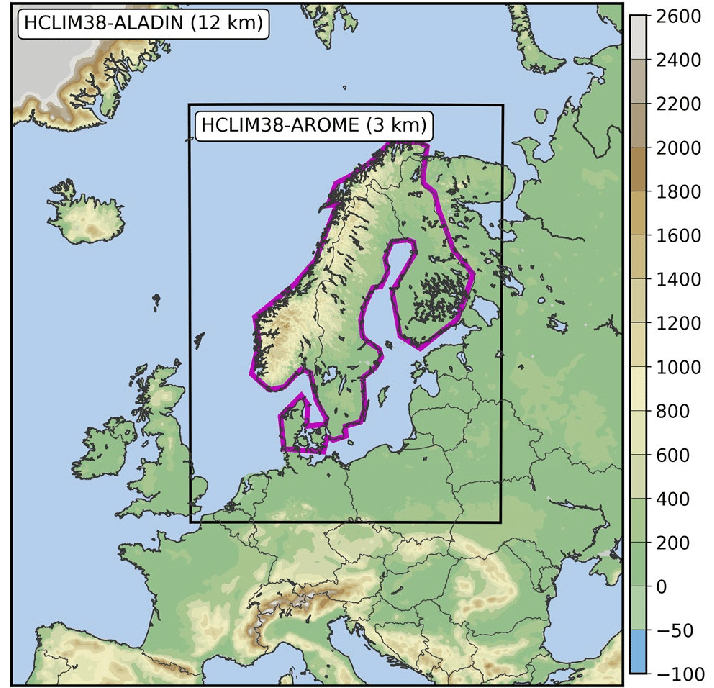
\includegraphics[scale=0.4]{figures/arome_domain.png}
    \caption{Domain used for HCLIM38-ALADIN (12km) simulation and domain used for HCLIM38-AROME (3km) simulation in the inner black rectangle. The colorscale represents the altitude above mean sea level in meters, and the magent colored area defines the Fenno-Scandinavian region. Source: Lind et al. 2020 \cite{lind_arome}}
    \label{fig:arome_domain}
\end{figure}

\subsubsection{AROME performance: an example}
Maybe an example showing how AROME have performed well on small-scale events and another on where it have performed poorly? 

\subsection{ting}

Anita: check annual maxima as well as returnvalues, might find some interesting info on why the return values are differeing between the methods